\section{カスタマイズ}

これ以降,``tsukuba-mas'' にあるオリジナルリポジトリ ``master\_report\_template'' を $A$ と呼びます.
また,$A$ のリポジトリを,あなたの GitHub リポジトリ に ``fork'' もしくは ``import'' したものを $B$ とします.
$B$ のリポジトリであなたの論文を書いていくことになります.

$A$ は,以下 URL で示されている学位論文テンプレートをカスタマイズしたものです.
よって,テンプレートにおけるすべての権利はシステム情報工学研究郡に帰属します.

\url{https://www.sie.tsukuba.ac.jp/visitor/student/thesis_after2020}

具体的には,以下のような変更が加えられています.

\begin{itemize}
    \item UTF-8 対応
    \item GitHub Actions 自動ビルド
    \item Make タスクツール
    \item textlint による自動校正
    \item components ファイル分割
\end{itemize}

\subsection{Clone}

あなたの論文をかくときには,$A$ のリポジトリを fork または import して
あなたのリポジトリに $B$ として追加してください.

論文を書く場合のおすすめは,import です.
$A$ に修正や機能追加などをする場合は,fork して PR を投げてもらえればうれしいです.

\begin{figure}[H]
    \centering
    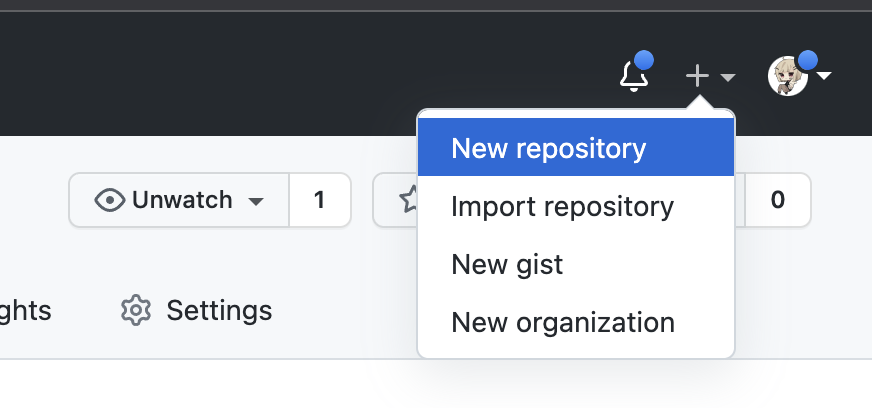
\includegraphics[width=0.5\linewidth]{static/introduction/import.png}
    \caption{$A$ を import する場合.}
\end{figure}

\subsection{GitHub Actions}

$A$ および $B$ には GitHub Actions が設定されています.
($A$ に設定されている GitHub Actions がそのまま $B$ にコピーされるためです.)
基本的な機能については,以下 2 つの記事で紹介しています.

\url{https://zenn.dev/ganariya/articles/platex-github-action}

\url{https://zenn.dev/ganariya/articles/weekly-paper-trial}

以下のような機能がついています.

\begin{itemize}
    \item Pull Request 時に textlint (後述) で文章校正テストを行う
    \item Git Tag を Push すると自動ビルドする
    \item 毎週決まった時間に自動ビルドする
    \item ビルド結果を Slack に通知する
\end{itemize}

ただし,Slack の機能を動作させるためには,$B$ のリポジトリで追加の設定が必要です.
\todo{Webhook URL の箇所が分かりづらいかも}
図\ref{fig:introduction_secrets}が示すように, ``Slack Webhook Incoming'' の URL を GitHub の Secrets に保存する必要があります.

\begin{figure}[H]
    \centering
    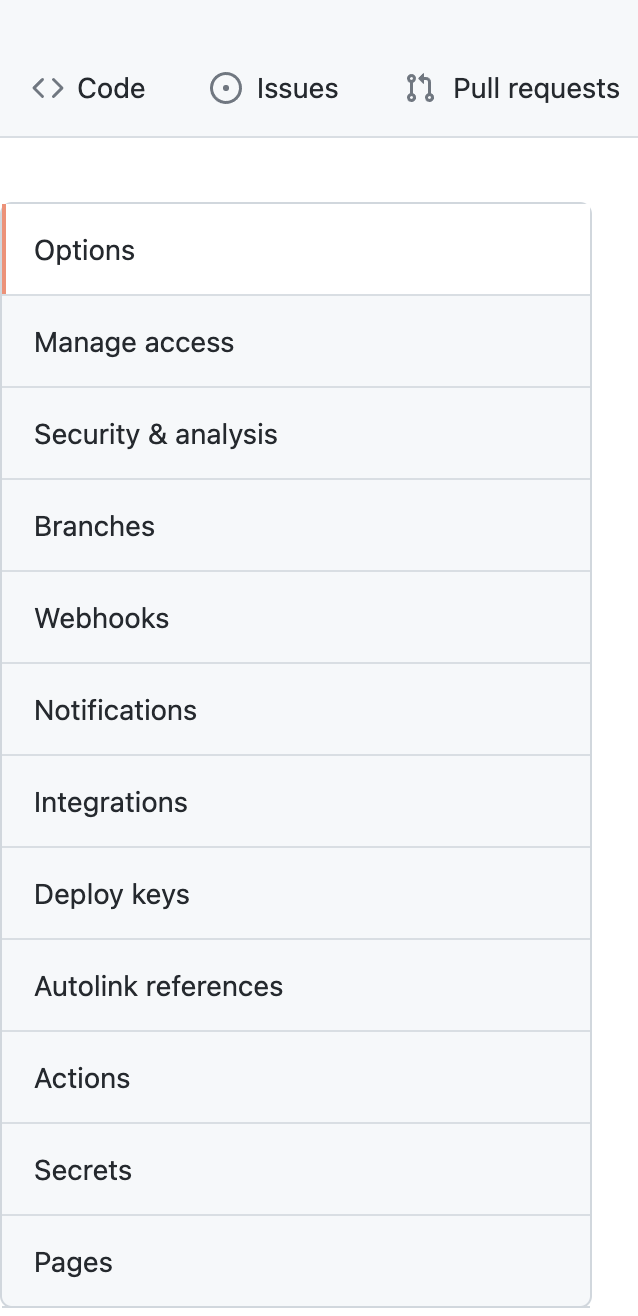
\includegraphics[width=0.3\linewidth]{static/introduction/secrets.png}
    \caption{GitHub Secrets}
    \label{fig:introduction_secrets}
\end{figure}

図\ref{fig:introduction_slack_webhook}が示すように,``SLACK\_WEBHOOK'' キーに,Webhook Incoming の URL を設定してあげてください.

\begin{figure}[H]
    \centering
    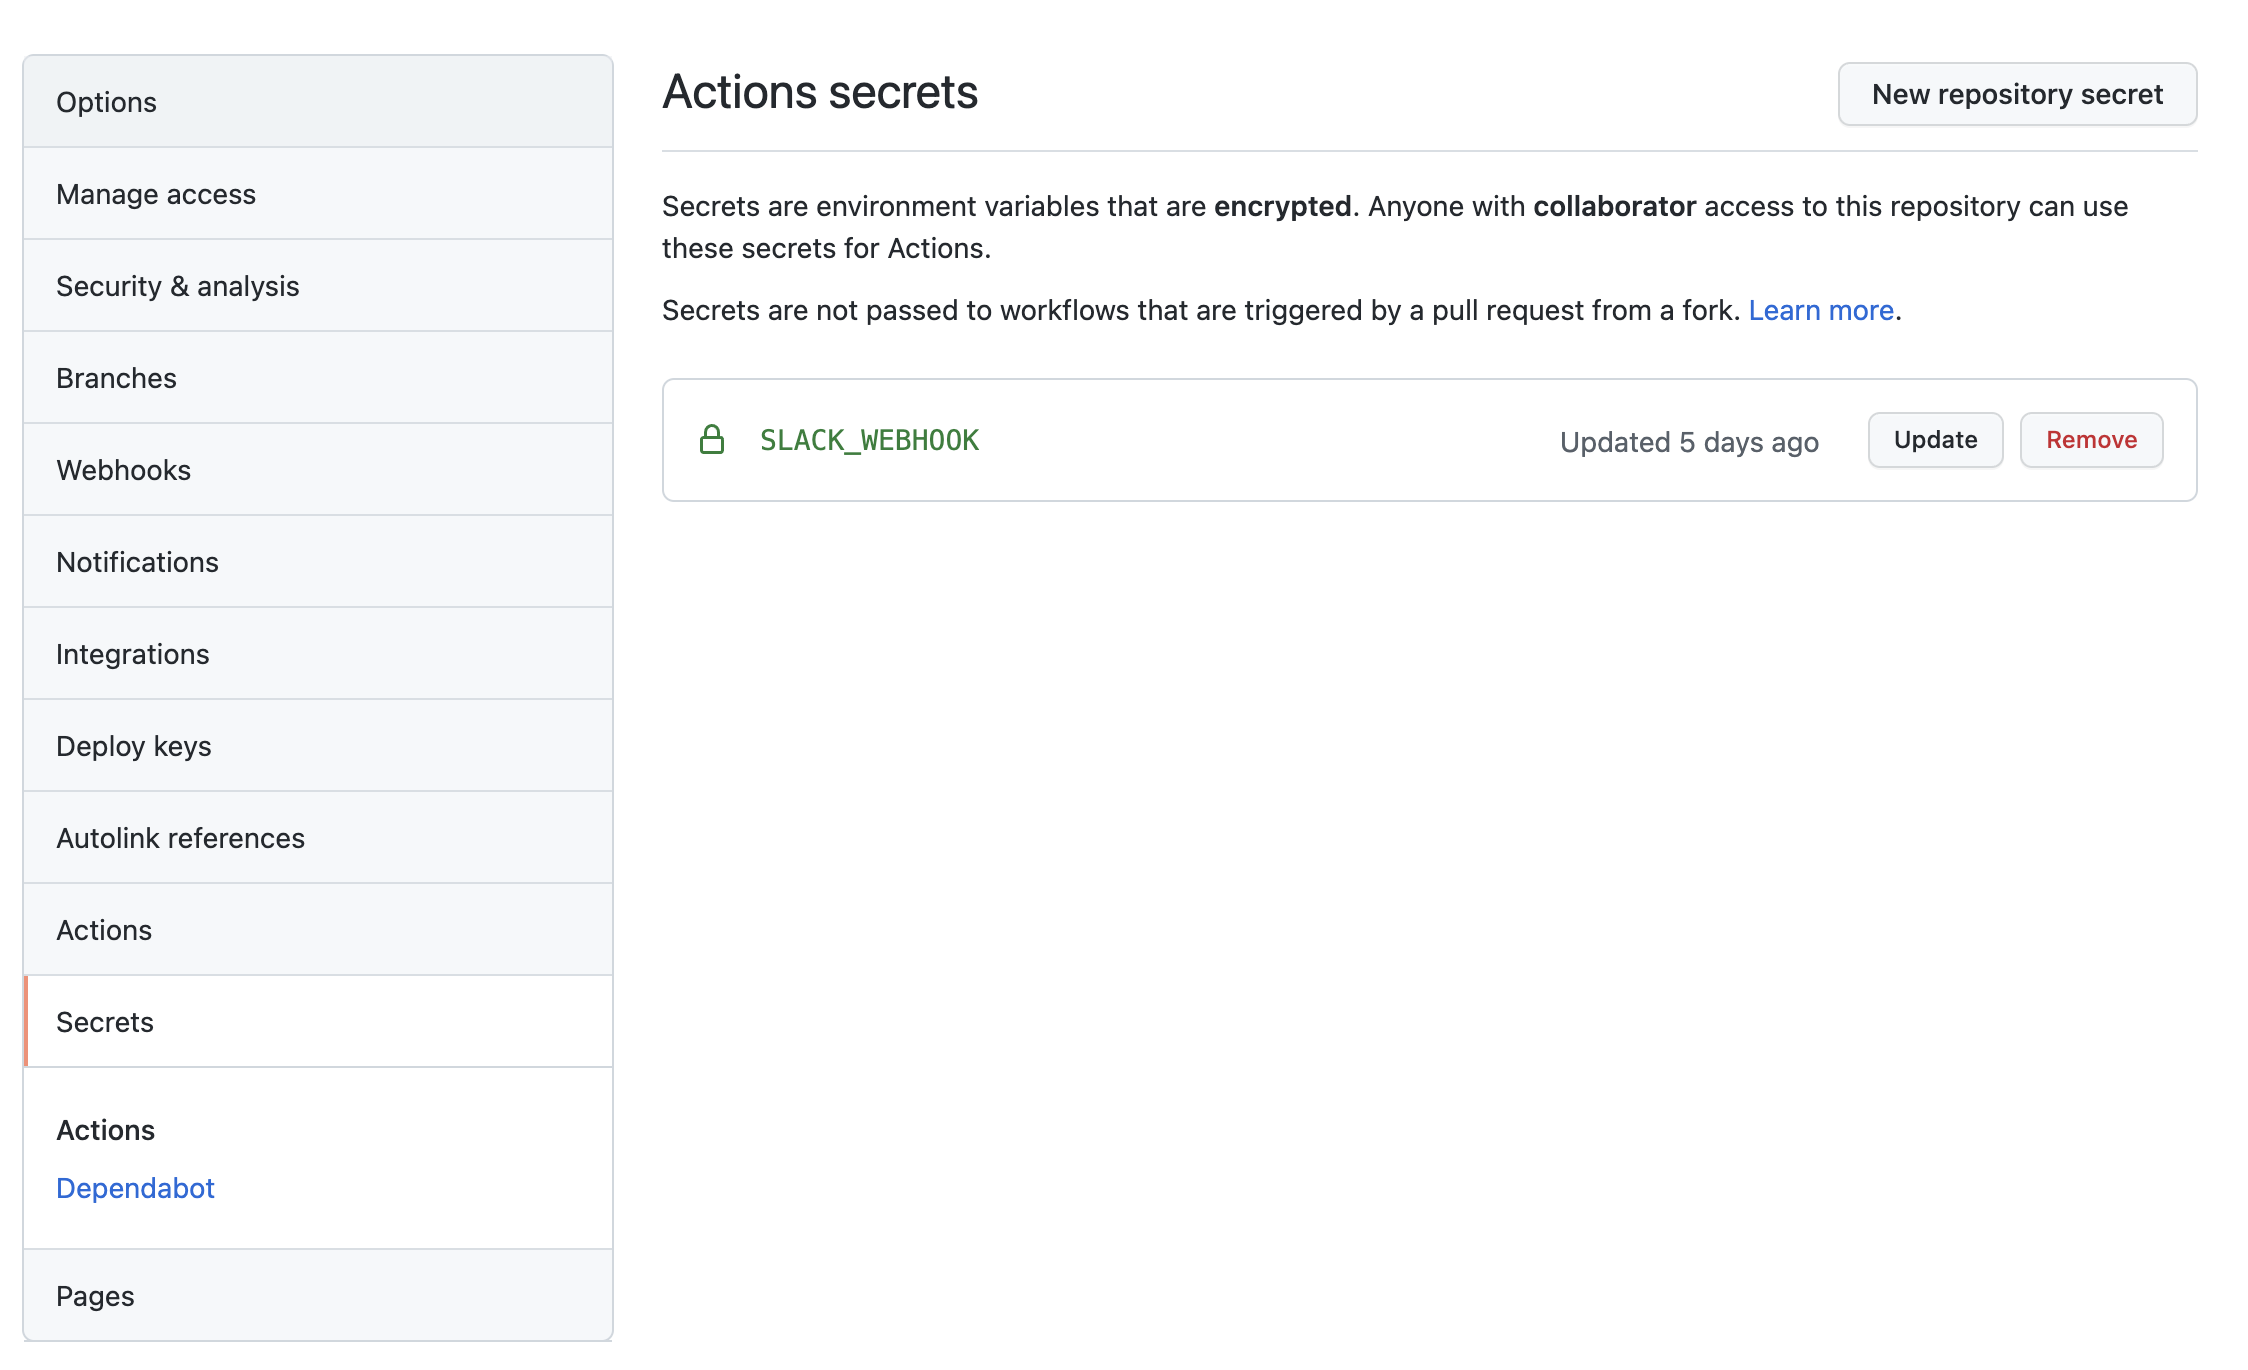
\includegraphics[width=0.6\linewidth]{static/introduction/slack_webhook.png}
    \caption{SLACK WEBHOOK}
    \label{fig:introduction_slack_webhook}
\end{figure}

\subsection{make}

Makefile が用意されています.
そのため,以下のようにコマンドを打つとコンパイルなどの処理が行えます.

とくに,textlint の機能を使うためには make install する必要があります.
make で行っている具体的な処理については Makefile を見てみてください.

\begin{lstlisting}[language=bash,caption={Makefile}]
# Install
make install

# compile
make compile

# clean
make clean
\end{lstlisting}

\subsection{textlint}

textlint というツールは,文章を自動校正してくれます.
自動校正の設定については,``.textlintrc'' で設定されています.
このファイルを変更することで,文章自動校正の設定を変更できます.

自動校正したいときは,``make lint'' などをすると良いです.
``make fix-lint'' することで,治せる部分は textlint が自動で修正してくれます.

ただし,textlint を使うためには,あらかじめ ``make install'' してください.
実質的には, ``npm install'' をしています.

\subsection{Welcome for Your Contributes}

% textlint-disable
修正や機能追加などのプルリクエストをお待ちしています!
% textlint-enable
